\documentclass{beamer}
\usetheme{manhattan}  % Now it's a beamer presentation with the Manhattan College theme!

\usepackage{url}
\usepackage{graphicx}
\usepackage{verbatim}
\usepackage{array}
\usepackage{amsthm, amsfonts, amsmath, amssymb, amsxtra}

\newcommand{\NP}{\ensuremath{\mathcal{NP}}}
% Make a new command that will make a new subsection and a frame with the same title
\newcommand{\fst}[2]{\subsection{#1}\frame{\frametitle{#1} #2}}

\title{Animation of Object-Oriented Program Execution}
\author{Peter Boothe}
\date{27 July 2011\\
BRIDGES 2011}
\institute[Manhattan College]{
    \url{peter.boothe@manhattan.edu}\\
    Mathematics and Computer Science \\
    Manhattan College}

\begin{document}
\frame{\titlepage}

\section{Why visualize execution}

\fst{Beautiful programs}{
\begin{center}
Programmers have long talked about art and style...\\
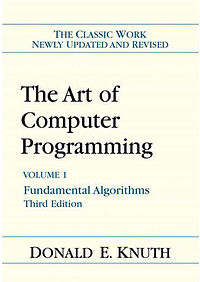
\includegraphics[height=.75in]{knuth.jpg}\ 
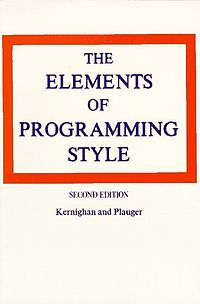
\includegraphics[height=.75in]{pstyle.jpg}
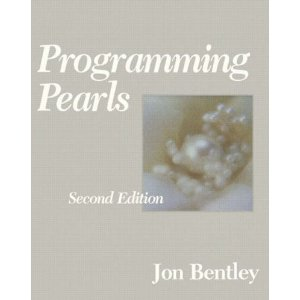
\includegraphics[height=.75in]{pearls.jpg}\ 
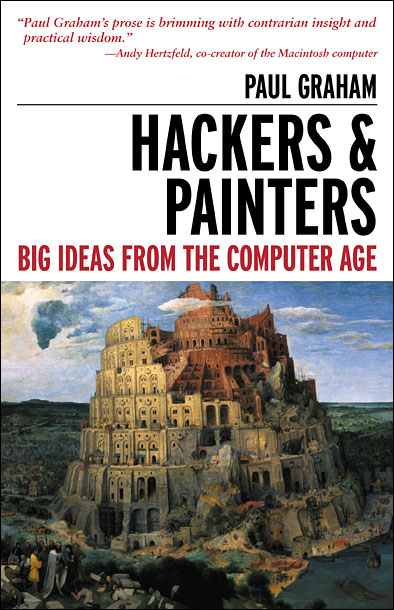
\includegraphics[height=.75in]{handp.jpg}\ 

Programmers are beginning to talk about beauty\\
\uncover<3->{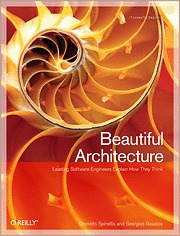
\includegraphics[width=.5in]{barch.jpg}}
\uncover<2->{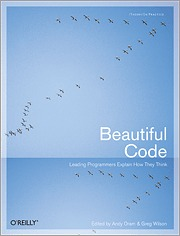
\includegraphics[width=.5in]{bcode.jpg}}
\uncover<6->{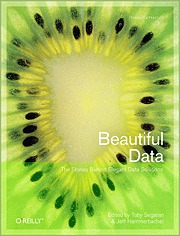
\includegraphics[width=.5in]{bdata.jpg}}
\uncover<5->{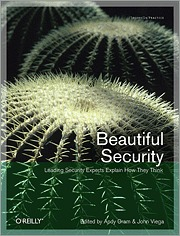
\includegraphics[width=.5in]{bsec.jpg}}
\uncover<4->{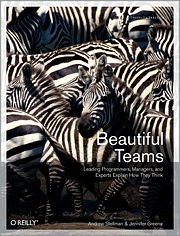
\includegraphics[width=.5in]{bteam.jpg}}
\uncover<7->{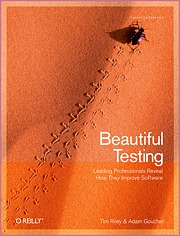
\includegraphics[width=.5in]{btest.jpg}}
\uncover<8->{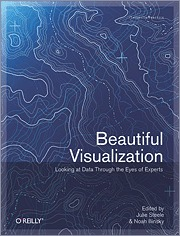
\includegraphics[width=.5in]{bvis.jpg}}
\end{center}

\uncover<8->{My claim:}
\uncover<9->{\LARGE \it The beauty of a program comes not from its source code, but from the unfolding of its execution.}
}

\fst{Programs are blueprints}{

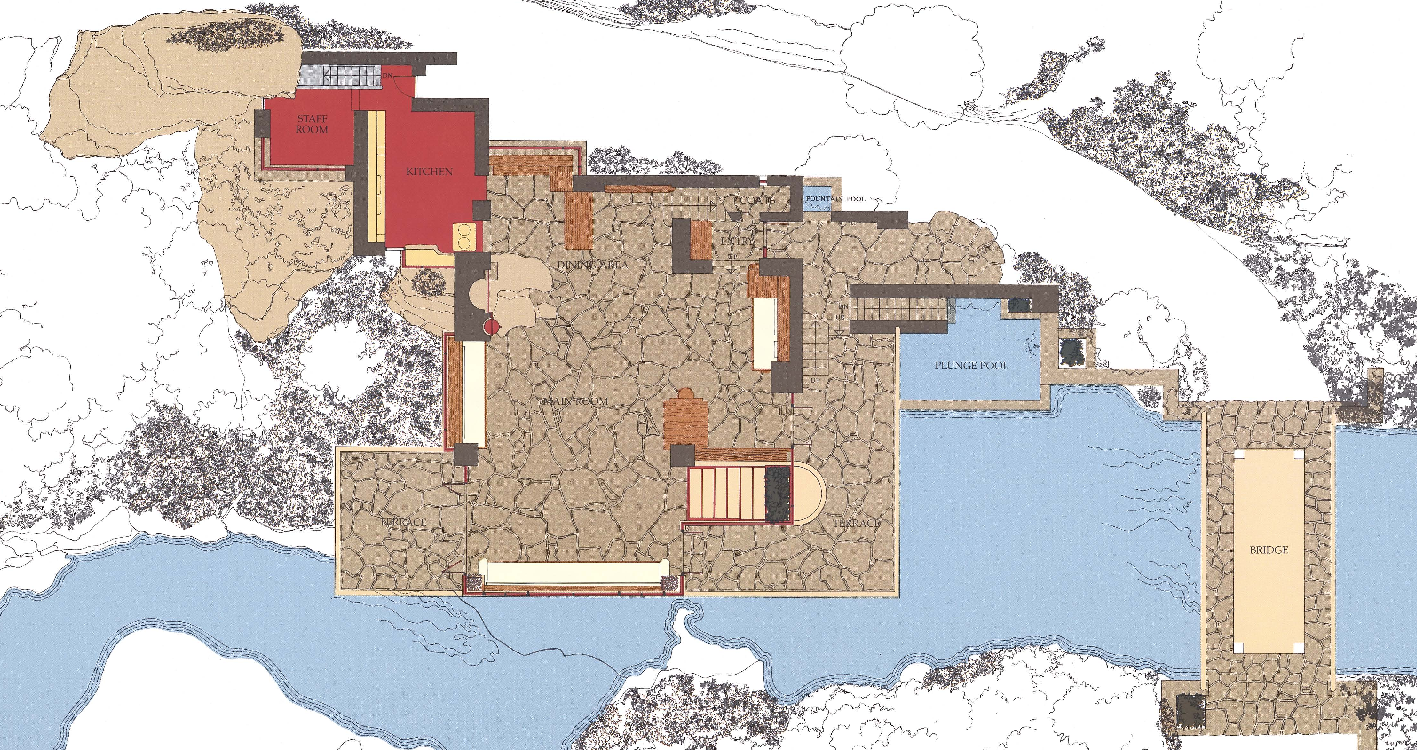
\includegraphics[width=4in]{fw.png}

}

\fst{The execution is what matters}{

\centering
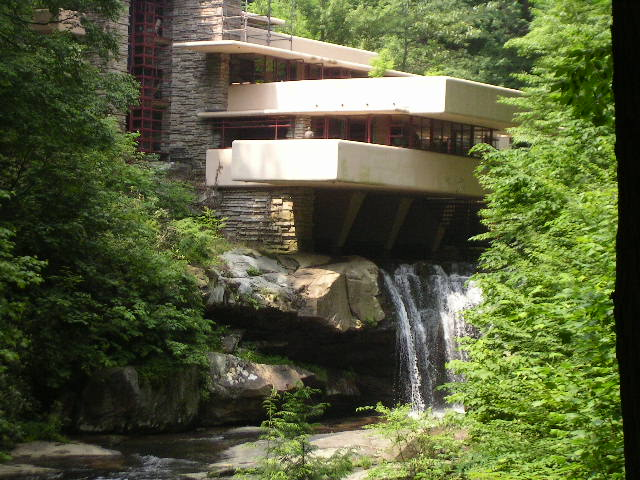
\includegraphics[width=3in]{fwpic.jpg}

{\tiny Thanks \url{http://www.fallingwater.org/assets/Site\%20Plan\%20and\%20Floor\%20Plans.pdf} and \url{http://www.flickr.com/photos/spike55151/14471574/}}
}

\section{Past Examples}

\fst{Atari Art}{
\begin{tabular}{c p{3in}}
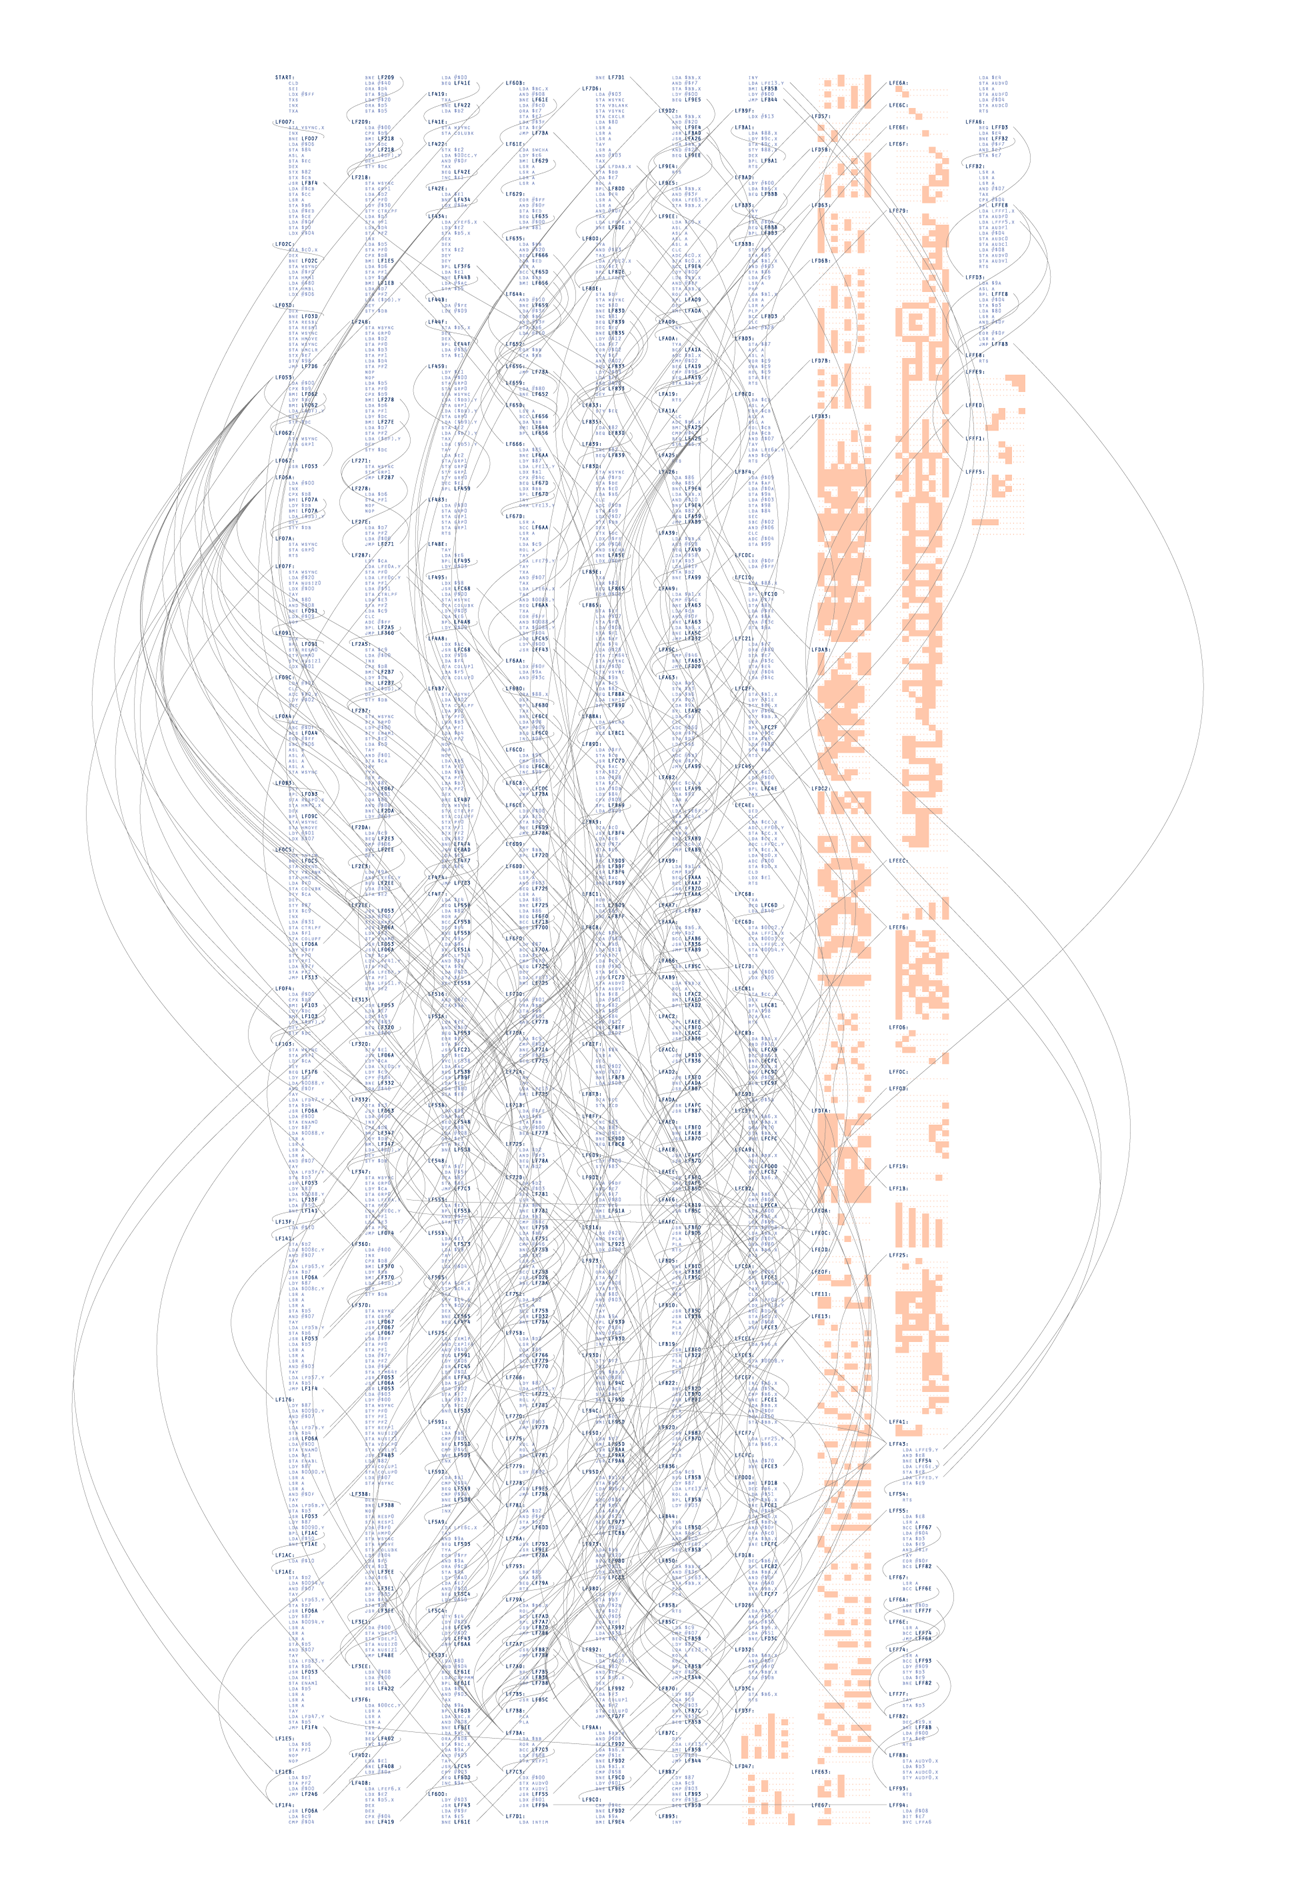
\includegraphics[height=2.75in]{pacman-illus-150dpi.png} &
\vspace{-2.5in}
\begin{itemize}
        \item Beautiful
        \item No execution
        \item Wrong level of abstraction
\end{itemize}
\vspace{1in}
\small{\url{http://benfry.com/distellamap/}}
\end{tabular}
}

\fst{Visual 6502}{
\begin{center}
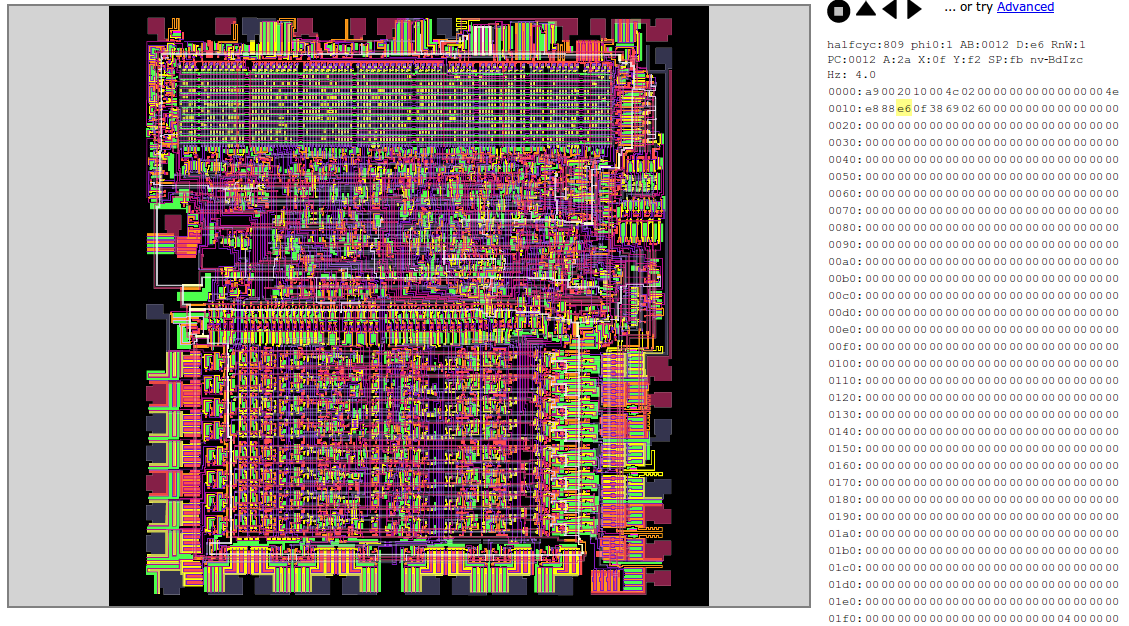
\includegraphics[height=2in]{6502.png}\\
Wrong level of abstraction.  Emphasizes hardware, not software.
\small{\url{http://http://visual6502.org/}}
\end{center}
}


\fst{Algorithm Visualization}{
\begin{tabular}{c p{2in}}
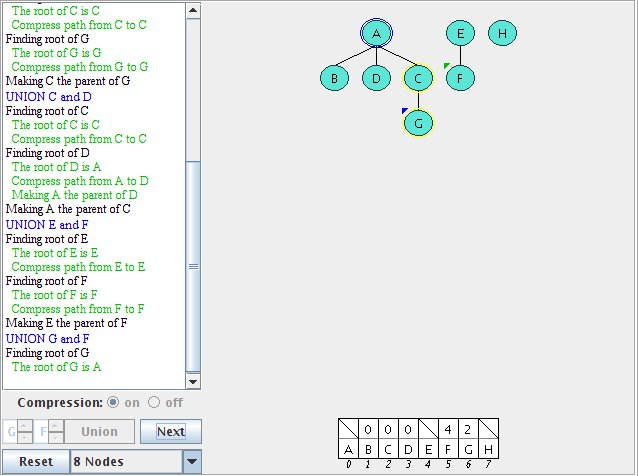
\includegraphics[width=2in]{algoviz.jpg} &
\vspace{-1.5in}
\begin{itemize}
\item Custom on a per-algorithm basis
\item Tricky to write
\item Not trying for beauty
\item Only one kind of beauty
\item Doesn't seem to help students learn, except for the students who write the visualization \cite{dandh}
\end{itemize}
\end{tabular}

Many more at \url{http://algoviz.org}

Picture is from \url{http://research.cs.vt.edu/AVresearch/UF/} 
}

\subsection{Lisp}
\frame[containsverbatim]{
\frametitle{Lisp and Trees}
\vspace{-.5in}
\begin{center}
\begin{tabular}{p{2in} p{.1in} p{2in}}
\begin{verbatim}
(((fun (f) (f f) ) 
  (fun (f) 
    (fun (n) 
     (if (< n 2) 1
      (* n ((f f) (- n 1)))
     )
    )
   )
 ) 6)
\end{verbatim} 
& \vspace{1in} 
$\to$ & \begin{figure}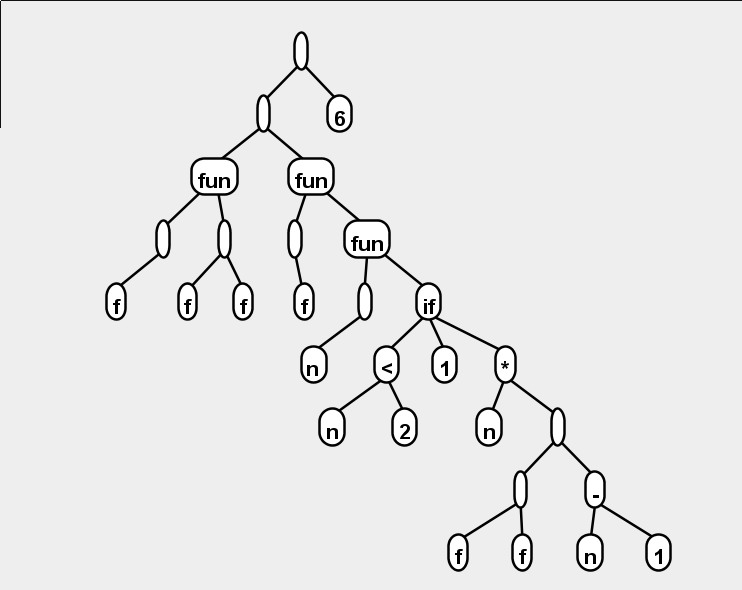
\includegraphics[width=2in]{fact.png}
\caption{Factorial program as a tree\cite{boca}}
\end{figure} \\
\end{tabular}

Animated, but requires programming in the visualizer.
\end{center}
}

\fst{Debuggers}{
\begin{center}
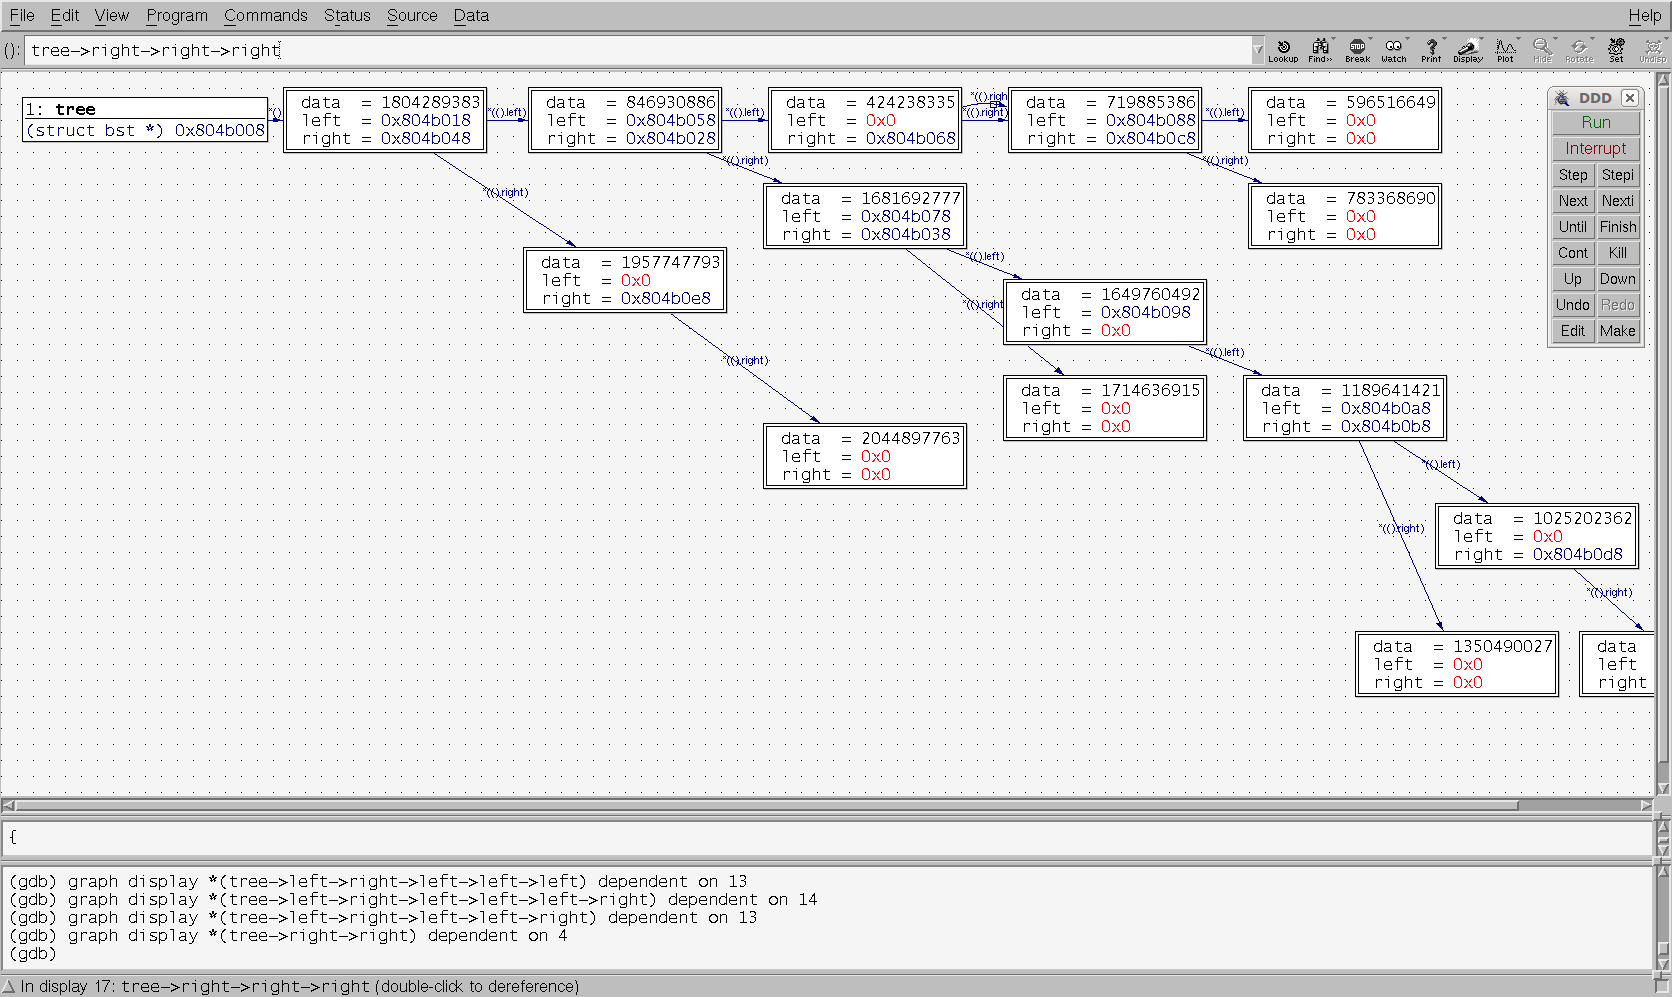
\includegraphics[width=3.75in]{ddd.png}

Not animated, beauty is ignored. \\
\tiny{(a DDD screenshot of a random binary search tree)}
\end{center}
}

\section{Animating a program}
\fst{Our goals}{
\begin{itemize}
        \item Look good
        \item Animate execution
        \item Be easy to use
        \item Show algorithmic beauty in our programs
        \item Show software engineering beauty
\end{itemize}
}
\fst{Program $\to$ Graph}{
\begin{itemize}
        \item Every object instance is a vertex
        \item Every stack frame is a vertex
        \item Every reference to an object constitutes a directed edge to an object
        \item Every function call constitutes a directed edge to a stack frame
        \item We use the debugging libraries to find all this information
\end{itemize}
}

\fst{Lay it out}{
    \begin{itemize}
        \item Use breadth-first search from {\tt main()} to generate a tree
        \item Same type $\to$ same type gets laid out in the XZ plane
        \item All other links are laid out in the XY plane
        \item XZ plane contains ``data structures'' elegance
        \item XY plane contains ``software design'' elegance
    \end{itemize}
}
\fst{Animate it}{
        \begin{itemize}
                \item Lay out the start
                \item Lay out the end
                \item Generate all of the tween frames
                \item Flip the flipbook
        \end{itemize}
}

\section{Demo}

\fst{Demo}{Here are a few programs, to end my talk.
\vspace{.5in}

All code (including all demos, slides, and the paper) may be freely downloaded
from \url{https://github.com/sbadame/Memeograph}}

\fst{Bibliography}{
        \bibliographystyle{apalike}
{\footnotesize 
        \bibliography{mybib}
}
}


\end{document}
